%
\comment{

1. Before performing any form of processing, a packet must be parsed in order to determine the header protocols
2. Various different combinations of protocols can be received --> this can be represented by a parsing graph
3. OpenFlow-based parsers have used match tables to traverse this graph: fields are matched with a certain entry in the table that contains information regarding which node to traverse to next
4. This model requires tables to contain all possible combinations of header protocols
5. Our key innovation replaces these tables with processing modules that are specific to one node in the parsing graph. Nodes that are small can be collapsed to form a larger node.
6. Nodes are interconnected using a full-crossbar
7. Full-crossbars are difficult to implement in FPGAs, as multiplexers do not synthesize well
8. Use the embedded NoC as the crossbar!!!

}
%

%

\figfull{2}{high-level-pp}{}{High level representation of module-based packet processor design. Packets are switched between processing modules corresponding to the protocols found in their headers.}

%\begin{figure}
%\centering
%%
%        \begin{subfigure}[t]{0.5\textwidth}
%        		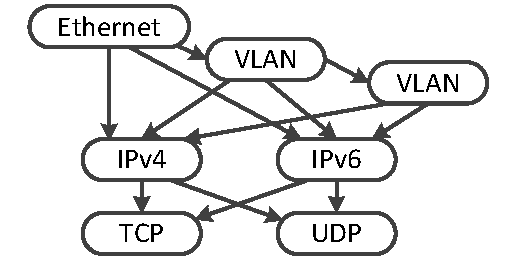
\includegraphics[width=\textwidth]{figs/parse-graph.pdf}
%        		\caption{Parse Graph}
%        		\label{parse-graph}
%		\end{subfigure}
%        \begin{subfigure}[t]{0.5\textwidth}
%        		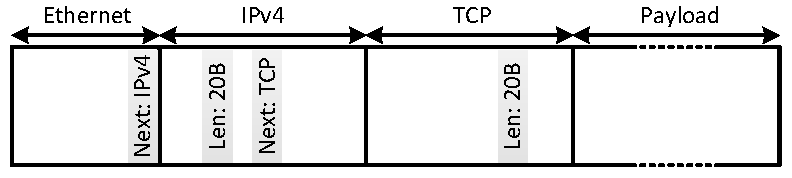
\includegraphics[width=\textwidth]{figs/packet.pdf}
%        		\caption{TCP/IP Packet}
%        		\label{packet}
%		\end{subfigure}
%\caption{An example parse graph commonly seen in enterprise networks, and a packet belonging to that parse graph. A parse graph can be used to represent the combinations of protocols that a packet processor may see in a certain application.}
%\label{parse-graph-packet}
%\end{figure}
%%
%
%Depending on the application, a packet processor must be able to process packets of a certain set of protocols.
%These protocols vary depending on the type of packet and layer they represent on the OSI stack.
%For example, Ethernet is one of the most common layer 2 protocols found in modern networks.
%The protocol at each layer contains information regarding the type and location of the protocol found in the next higher layer (Figure~\ref{packet}).
%The various different combinations of protocols that may be received in a single packet can be represented by a parsing graph~\cite{gibb2013design} (Figure~\ref{parse-graph}).
%
%As network protocols are changed, added and replaced, a programmable packet processor must be able to be reconfigured to support different parsing graphs.
%OpenFlow-based processors use match tables to traverse these graphs.
%When a field is matched at a table entry for a protocol at a certain OSI stack layer, the entry contains information regarding where to look in the next match table for the protocol of the next layer.
%This model requires match tables to contain all possible combinations of header protocols and field values that the processor may face.

%
%\begin{figure}[t] \centering
%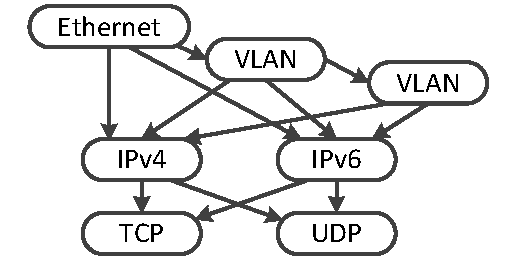
\includegraphics[width=0.35\textwidth]{figs/parse-graph.pdf}
%\caption{An example parse graph commonly seen in enterprise networks. A parse graph can be used to represent the combinations of protocols that a packet processor may see in a certain application.}
%\label{parse-graph}
%\vspace{0cm}
%\end{figure}
%

Instead of match tables that each support a set of protocols, our design implements multiple processing modules, with each module dedicated to processing a single parsing graph node's protocol (Figure~\ref{parse-graph}).
Packets are sent to the modules corresponding to the protocols found in their headers.
Each processing module determines what actions to take for its protocol, and the type and location of the protocol processing module for the packet's next OSI layer.
%For example, consider a packet consisting of Ethernet, IPv4, and TCP headers (as in Figure~\ref{packet}).
%Such a packet would first be forwarded to an Ethernet processing module, where it would be discovered that the protocol of the next header is IPv4.
%Once Ethernet processing is complete, the packet would then be sent to an IPv4 processing module, and finally to a TCP processing module.
%Another packet containing Ethernet, IPv6, and TCP headers would follow nearly the same path, except instead of being sent to an IPv4 processing module, it would be sent to one for IPv6.
Figure~\ref{high-level-pp} depicts a general representation of this packet processor design.

The FPGA reconfigurable fabric is used to implement the processing modules.
The flexibility of the fabric allows for the modules to be fully customized and later updated, as existing protocols are enhanced and new protocols are added.
It is by updating the modules that processing rule updates are made.
For example, in order to modify the supported parse graph, each module's routing decision logic is updated to match the new set of edges connecting its corresponding node in the graph.
Module updates are made by reconfiguring (or partially reconfiguring, see Section~\ref{sec:reconfig}) the FPGA.

%As in any packet processor, the processing modules perform some set of actions when packet fields are matched.
%However, since each processing module is dedicated to a single node in the parsing graph, its matches and actions are tied solely to what is relevant to that node.
%It is by updating the modules that processing rule updates are made.
%Field matches, actions, routing decision logic 
%In order to modify the supported parse graph, each module's routing decision logic is updated to match the new set of edges connecting its corresponding node in the graph.
%Field matches and routing decisions at a particular protocol node can be stored in tables at the module.
%These tables only need to contain entries relevant to actions that can take place for that protocol, unlike the OpenFlow flow tables, which must have entries for all possible field matches at that stage.
%In effect, a flow table is broken up and spread across several processing modules.
%The module tables' widths and depths, as well as the modules actions, can be customized to fit only the module's protocol.
%We argue that having these ``fine-grained'' tables that are specifically customized for a protocol will allow for a more efficient design than OpenFlow's ``coarse-grained'' flow tables.
%For example, an OpenFlow flow table that is expecting either IPv4 and IPv6 packets must be made wide enough to match the 128-bit address fields of IPv6, despite the fact that IPv4 addresses are only 32 bits.
%If there are many more IPv4 addresses to be matched, then the table would also have to be deep enough to hold all the address entries.
%In contrast, our design would have an IPv4 module with a match table that is deep enough to hold all the entries, but only need to be wide enough to hold the 32-bit addresses.
%Similarly, the IPv6 module table could be made shallow and wide.


Interconnecting the processing modules is a challenging problem on current FPGA devices.
Multiplexers, which are necessary for the full crossbars in Figure~\ref{high-level-pp}, are synthesized poorly on the FPGA's fabric, often consuming relatively high chip area and running considerably slower than they would if built in ASIC technology.
A full crossbar that is wide enough to support the very high bandwidth of data entering modern packet processors would be very difficult, if not impossible, to efficiently synthesize in the FPGA fabric.

%Besides module duplication, the NoC-PP design also allows for the easy addition and/or removal of protocols as needed.
%Say a new protocol has been developed and must be supported by the packet processor.
%A processing module for this protocol can then be designed and added to the NoC-PP by connecting it to any of the routers in the NoC, with little other modification to the rest of the design.
%Similarly, if a protocol no longer needs to be supported, then its processing modules can simply be removed from the design.

